\documentclass[a4paper, 11pt]{article}
\usepackage{comment} % enables the use of multi-line comments (\ifx \fi) 
\usepackage{lipsum} %This package just generates Lorem Ipsum filler text. 
\usepackage{fullpage} % changes the margin
\usepackage{fancyhdr}
\usepackage{lmodern} % police propre
\usepackage[utf8]{inputenc}
\usepackage[T1]{fontenc}
\usepackage[francais]{babel}
\usepackage{graphicx}
\usepackage{listings}

\usepackage{color}
 
\definecolor{codegreen}{rgb}{0,0.6,0}
\definecolor{codegray}{rgb}{0.5,0.5,0.5}
\definecolor{codepurple}{rgb}{0.58,0,0.82}
\definecolor{backcolour}{rgb}{0.95,0.95,0.92}
 
\lstdefinestyle{mystyle}{
    backgroundcolor=\color{backcolour},   
    commentstyle=\color{codegreen},
    keywordstyle=\color{magenta},
    numberstyle=\tiny\color{codegray},
    stringstyle=\color{codepurple},
    basicstyle=\footnotesize,
    breakatwhitespace=false,         
    breaklines=true,                 
    captionpos=b,                    
    keepspaces=true,                 
    numbers=left,                    
    numbersep=5pt,                  
    showspaces=false,                
    showstringspaces=false,
    showtabs=false,                  
    tabsize=2
}
 
\lstset{style=mystyle}

\usepackage{sectsty}
\sectionfont{\fontsize{12}{15}\selectfont}

\usepackage{geometry}
\geometry{hmargin=1.5cm,vmargin=1.5cm}

\begin{document}
%Header-Make sure you update this information!!!!
\noindent
Pierre Berard, Florian Perroud, Alexandre Rupp  \hfill 30/11/2015 
%\vspace{0.01cm}
\vspace{-0.3cm}\\

{\LARGE 
\begin{center}
\textbf{Gestion de Données à Grande Echelle} \\
\vspace{0.2cm}
\end{center}
}
\begin{center}
\textbf{NoSQL assignment} \\
\end{center}

%Introduction
%Personal experience
%Problem encontered
%Solutions
%Athmoshpere at work
%Management relations
%Conclusion


\section{Introduction}
The database represents the data to be used by a MMORPG \footnote{MMORPG: Massively Multiplayer Online Role Playing Games.}.
The game is composed of users, each user can have at most 5 characters. A character has a race, has weapons, may belong to a team and is moving on a map.

\section{Data Stored in Database}

\begin{figure}[!h]
  \centering
  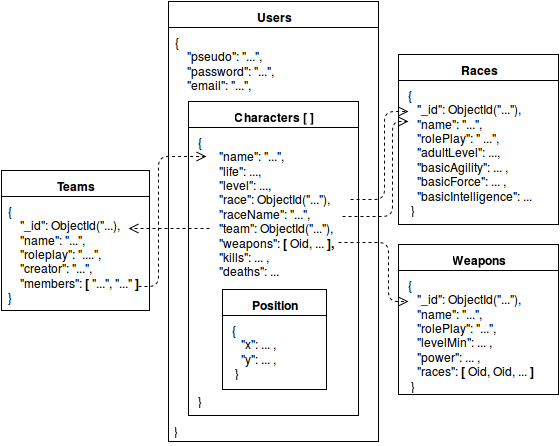
\includegraphics[width=0.7\linewidth]{MMORPG_schema.png}
    \caption{Schéma de la base de donnée}
\end{figure}

\paragraph{Users and Characters:} the document \textit{User}, contains a list of \textit{Characters}. The relationship between the two is of type 1 - N (or more precisely: 1-Few). It has been chosen to embed the characters in the user document, since we often need the 2 together. Furthermore, a user can only have a few (max 5) characters (so the limit of 16MB per document will not be reached). Then, a character can not be shared by multiple users. In this case, the best solution was to embed it in the User table.

\paragraph{Character and Position:}
The Position document is small, never accessed alone, and may be shared by multiple users (in a few cases). The relationship between Character and Position is N-1, but most of the positions on the map are empty. Most of the time, the application wants to know the position of the current player, and also what players are in the near area. In this case, we decided to fully embed the document Position in Character.

\paragraph{Character and team:}
The relationship between the two is N-1 (more precisely: Few-1). A team can be accessed alone and therfore, we could not embed it (moreover, it would have implied a lot of redundancy).\\
The relationship is two-way, because when selecting a character we want to know his team and when we select a team we want to know its members.
In order to optimize it, we have added a reference to the team in Character and a list of members in team.

\paragraph{Character and weapons:}
This is a N-N relationship. Weapons may be accessed standalone (for example in the shop), thus it could not be embedded. Most of the time, we want to know the weapons of a character (never in the opposite way). For these reasons, a Character contains a list of weapons references.

\paragraph{Character and race:}
This is a 1-N relationship. Races contains different characteristics and it would be costly to embed it in characters. Races may be accessed standalone (list of races). Most of the time, we need to know the race of a character. We never want to know all the characters of a race. Thus, it is a one way relationship. Therefore, a character contains a ref to his race. \\
Most of the time, when we access a character, we want to access the name of his race, that is why we added the name of the race in the Character document (denormalisation). This decision increases the speed of the read, and dicreases the updates. This is a good decision because the races are barely never updated.




\section{Indexes}
And index has been created on User pseudos, since most of the time, users are accessed by there pseudo.\\
It is the same thing for the names of characters, weapons, races and teams.
There is also an index on characters.team.

\section{Queries}
\paragraph*{Query 1\\}
The first query is to find the characters on the map who are around our character. In order to do so, we execute a first request to get the position of the character we are playing with. Then we find all the players present in a 11 square area around the character position.

\begin{lstlisting}
// Find my user profile : 
var me = db.users.findOne({pseudo: ``tchoubid0o''});

// 1) Find other characters around my character:
var myCharacter = me.characters[0];
var myPos = myCharacter.position;
db.users.aggregate([
    {$unwind: ``$characters''}, 
    {$match: 
     {$and: 
      [
          {``characters.name'': {$ne: myCharacter.name}},
          {``characters.position.x'': {$gte: myPos.x-5}}, 
          {``characters.position.x'': {$lte: myPos.x+5}}, 
          {``characters.position.y'': {$gte: myPos.y-5}}, 
          {``characters.position.y'':{$lte: myPos.y+5}}
      ]
     }
    },
    {$project: {_id: 0, character: ``$characters''}}
]);
\end{lstlisting}

Here the index on user's pseudo is involved. It enables us to find the player faster.

\paragraph*{Query 2\\}
The second query is used to find the best weapon that a character has and cas use. For this character, we find all the weapons he has and can use, according to his level and race. Those weapons are then ordered by power, and we keep the first one.
~\\
~\\
\begin{lstlisting}
var characterName = 'Elfounet';
var character = db.users.aggregate([
    {$unwind: "$characters"}, 
    {$match: {"characters.name": characterName}},
    {$project: {_id: 0, character: "$characters"}}
]).result[0].character;

db.weapons.find({_id: {$in: character.weapons}, 
                 levelMin: {$lte: character.level}, 
                 races: character.race
                });
\end{lstlisting}

In this case, no index is used.

\paragraph*{Query 3\\}
This query is used to obtain a sorted list of the 3 characters having the best kill/death ratio. To do so, we unwind the array of characters, we realize a projection to work out the ratio per player and finally we sort the list by ratio and keep the 3 first characters (limit).

\begin{lstlisting}
db.users.aggregate([
    {$unwind: ``$characters''}, 
    {$project: {_id: 0, 
                name: ``$characters.name'', 
                ratio: {$divide: [``$characters.kills'', ``$characters.deaths'']}
               }
    },
    {$sort: {ratio: -1}},
    {$limit: 3}
]);
\end{lstlisting}

In this case, no index is used.

\paragraph*{Query 4\\}

This query is used to obtain the details concerning the best team of the game (i.e. the one having the best average of ratio per player).
To do so, we unwind the list of characters, we match those belonging to a team, we realize a projection to work out the ratio per player, we do a group to work out the average ratio per team and finally we sort and limit to get the best team.

\begin{lstlisting}
var bestTeam = db.users.aggregate([
    {$unwind: ``$characters''}, 
    {$match: {``characters.team'': {$exists: 1}}},
    {$project: {_id: 0, name: ``$characters.name'',
                team: ``$characters.team'', 
                ratio: {$divide: [``$characters.kills'', ``$characters.deaths'']}
               }
    },
    {$group: {_id: ``$team'', average_ratio: {$avg: ``$ratio''}}},
    {$sort: {average_ratio: -1}},
    {$limit: 1}
]);
\end{lstlisting}

In this case, the index on characters.team is used in the match close.

\paragraph*{Query 5\\}
This query is used to find the most used race among the existing characters. To do so, we group the character by their raceName and count them. Then we keep only the first one.

\begin{lstlisting}
db.users.aggregate([
    {$unwind: "$characters"},
    {$group: {_id: "$characters.raceName", count: {$sum: 1}}},
    {$sort: {count: -1}},
    {$limit: 1}
]).result[0]._id;
\end{lstlisting}

In this case, no index is used.

\end{document}

